\documentclass{ctexart} % 子文件也要声明类型

% === 引入公共配置 ===
% 这样单独编译时,它就有颜色和代码高亮了
\usepackage{my_style} 

\begin{document} 
% 注意:主文件读取时,会忽略上面的所有内容,直接从这里开始读取

\section{[CSP-J 2025] 座位 / seat} 

\subsection*{题目描述}
CSP-J 2025 第二轮正在进行。小 R 所在的考场共有 $n \times m$ 名考生,其中所有考生的 CSP-J 2025 第一轮成绩互不相同。所有 $n \times m$ 名考生将按照 CSP-J 2025 第一轮的成绩,由高到低蛇形分配座位,排列成 $n$ \textbf{行} $m$ \textbf{列}。具体地,设小 R 所在的考场的所有考生的成绩从高到低分别为 $s_1 > s_2 > \dots > s_{n \times m}$,则成绩为 $s_1$ 的考生的座位为第 1 \textbf{列}第 $1$ \textbf{行},成绩为 $s_2$ 的考生的座位为第 $1$ \textbf{列}第 $2$ \textbf{行},$\dots$,成绩为 $s_n$ 的考生的座位为第 $1$ \textbf{列}第 $n$ \textbf{行},成绩为 $s_{n+1}$ 的考生的座位为第 $2$ \textbf{列}第 $n$ \textbf{行},$\dots$,成绩为 $s_{2n}$ 的考生的座位为第 $2$ \textbf{列}第 $1$ \textbf{行},成绩为 $s_{2n+1}$ 的考生的座位为第 $3$ \textbf{列}第 $1$ \textbf{行},以此类推。

例如,若 $n = 4, m = 5$,则所有 $4 \times 5 = 20$ 名考生将按照 CSP-J 2025 第一轮成绩从高到低的顺序,根据下图中的箭头顺序分配座位。

\begin{figure}[h]
\centering
\includegraphics[width=0.6\textwidth]{image}
\caption{蛇形排列示意图($n=4, m=5$)}
\end{figure}

\subsection*{输入输出格式}
\textbf{输入:}第一行,两个正整数 $n, m$,分别表示考场座位的\textbf{行数}与\textbf{列数}。\par
\qquad\quad 第二行,$n \times m$ 个正整数 $a_1, a_2, \dots, a_{n \times m}$,表示所有考生 CSP-J 2025 第一轮的成绩,其中 $a_1$ 为小 R 的成绩。\par
\textbf{输出:}一行两个正整数 $c, r$,表示小 R 的座位为第 $c$ \textbf{列}第 $r$ \textbf{行}。

\begin{table}[h]
\centering
\begin{tabularx}{\textwidth}{|X|X|}
\hline
\textbf{输入示例} & \textbf{输出示例}     \\    
\hline
2 2 & 1 2   \\ 
99 100 97 98 & \\ 
\hline
2 2 & 2 2   \\ 
98 99 100 97 & \\ 
\hline
3 3 & 3 1   \\ 
94 95 96 97 98 99 100 93 92 & \\ 
\hline
\end{tabularx}  
\end{table}

\subsection*{样例解释}
\textbf{样例1:}成绩从高到低排序为:100, 99, 98, 97。

座位分配过程如下图所示:
\begin{figure}[h]
\centering
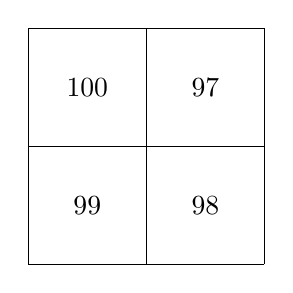
\begin{tikzpicture}[scale=1.5]
\draw (0,0) grid (2,2);
\node at (0.5,1.5) {100};
\node at (0.5,0.5) {99};
\node at (1.5,0.5) {98};
\node at (1.5,1.5) {97};
\end{tikzpicture}
\caption{样例1座位分配图(n=2, m=2)}
\end{figure}

小 R 的成绩为99,位于第1列第2行。

\textbf{样例2:}成绩从高到低排序为:100, 99, 98, 97。

座位分配与样例1相同,分配图如下:
\begin{figure}[h]
\centering
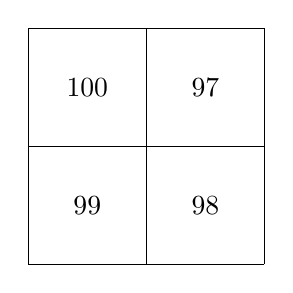
\begin{tikzpicture}[scale=1.5]
\draw (0,0) grid (2,2);
\node at (0.5,1.5) {100};
\node at (0.5,0.5) {99};
\node at (1.5,0.5) {98};
\node at (1.5,1.5) {97};
\end{tikzpicture}
\caption{样例2座位分配图(n=2, m=2)}
\end{figure}

但小 R 的成绩为98,因此座位为第2列第2行。

\subsection*{算法分析}
\begin{enumerate}
\item \textcolor{important}{\textbf{问题转化}}\\
本题的核心在于按照\textcolor{important}{\textbf{蛇形顺序}}填充矩阵,并找到目标成绩的坐标。首先,我们需要将所有考生的成绩\textcolor{important}{\textbf{从大到小排序}}。

\item \textcolor{important}{\textbf{规律观察}}\\
观察题目给出的蛇形排列方式,我们可以发现\textbf{列的奇偶性}决定了行的填充方向:
 \begin{enumerate}
    \item \textbf{奇数列(第1, 3, 5...列)}:成绩从\textcolor{important}{\textbf{上到下}}(行号 $1 \to n$)依次排列。
    \item \textbf{偶数列(第2, 4, 6...列)}:成绩从\textcolor{important}{\textbf{下到上}}(行号 $n \to 1$)依次排列。
 \end{enumerate}

\item \textcolor{important}{\textbf{算法步骤}}
 \begin{enumerate}
    \item 记录小 R 的原始成绩(输入数组的第一个数)。
    \item 对成绩数组进行降序排序。
    \item 使用一个全局指针 `idx` 指向排序后的成绩数组。
    \item \textcolor{important}{\textbf{外层循环}}枚举列号 $c$ 从 $1$ 到 $m$:
    \begin{itemize}
        \item 若 $c$ 为奇数,\textcolor{important}{\textbf{内层循环}}行号 $r$ 从 $1$ 到 $n$;
        \item 若 $c$ 为偶数,\textcolor{important}{\textbf{内层循环}}行号 $r$ 从 $n$ 到 $1$。
    \end{itemize}
    \item 在填充过程中,比较当前填入的成绩是否等于小 R 的成绩。若相等,立即输出当前的 $(c, r)$ 并结束程序。
 \end{enumerate}

\end{enumerate}

\subsection*{参考代码}
\begin{lstlisting}
#include "bits/stdc++.h"
using namespace std;
using u32 = unsigned;
using i32 = int;
using u64 = unsigned long long;
using i64 = long long;
using u128 = unsigned __int128;
using i128 = __int128;

#define int long long
#define endl "\n"

constexpr i64 inf = 1e18;

void slu() {
    int n, m;
    cin >> n >> m;
    vector<int> a(n * m);
    for (auto& x : a) cin >> x;
    int aim = a[0];
    sort(a.begin(), a.end(), greater());
    vector<vector<int>> M(n, vector<int>(m, 0));

    int x = 0, y = 0;
    int T = 0;
    int cur = 0;
    while (x < n && y < m) {
        M[x][y] = a[cur++];
        if (M[x][y] == aim) {
            cout << y + 1 << "` `" << x + 1;
            return;
        }
        if (T < n - 1) x++;
        else if (T == n - 1) y++;
        else if (T != 2 * n - 1) x--; 
        else y++;
        
        T = (T + 1) % (2 * n);
    }
}

signed main() {
    ios_base::sync_with_stdio(false);
    cin.tie(nullptr);
    cout.tie(nullptr);

    int t = 1;
    // cin >> t;

    while (t--) slu();
    return 0;
}
\end{lstlisting}

\subsection*{拓展思考}
\begin{itemize}
    \item \textcolor{important}{\textbf{数学推导($O(1)$ 解法)}}:
    假设小 R 的成绩在排序后排在第 $k$ 名(下标从 0 开始)。
    \begin{enumerate}
        \item 所在的列号:$c = k / n + 1$。
        \item 所在的行号:
        \begin{itemize}
            \item 若 $c$ 为奇数,行号 $r = (k \% n) + 1$;
            \item 若 $c$ 为偶数,行号 $r = n - (k \% n)$。
        \end{itemize}
    \end{enumerate}
    这种方法无需模拟整个矩阵,效率更高。
    \begin{lstlisting}
int n, m;
cin >> n >> m;
vector<int> a(n *m);
for (auto &x : a) cin >> x;

int target = a[0];
sort(a.begin(), a.end(), greater<int>());

int idx = -1;
for (int i = 0; i < n * m; i++) {
    if (a[i] == target) {
        idx = i;
        break;
    }
}

int c = idx / n + 1;
int r;
if (c % 2 != 0) {
    r = (idx % n) + 1;
} else {
    r = n - (idx % n);
}

cout << c << "` `" << r << endl;
    \end{lstlisting}
\end{itemize}

\end{document}